\chapter[Introdução]{Introdução}
\label{ch:introdução}
A eletricidade se tornou um pilar central na atualidade, sendo uma das principais fontes de força, calor e luz utilizada no  mundo. Entrantando com o
crescente consumo de energia elétrica nos últimos tempos, a demanda por produção da mesma teve um crecismento significativo, trazendo consigo 
impactos ambientais e econômicos. O Brasil por mais que possua em seu território grandes possibilidade para a construção de hidrelétricas, não
está isento do problema da alta demanda por energia elétrica. Problema que se agravou em 2015 quando o país começou a passar por
uma crise hídrica.

Como a \autoref{fig:rede_convencional} mostra, a maior parte da energia elétrica gerada no Brasil é por meio de hidroelétricas, essa dependência
energetica junto com a crise hídrica que o país sofreu cuminou em uma política de racionamento e aumento dos impostos - taxa inflacionária no
consumo de energia elétrica - que impactou diretamente a vida de cada cidadão brasileiro, trouxe consequências, como o aumento do 
custo da energia elétrica. Segundos dados (G1, 2016) entre 2015 e 2016 a crise hídrica no Brasil não interferiu apenas na conta de luz mas trouxe
um aumento na inflação do país.

% sustentabilidade


% JONATHAN aqui seu capítulo introdutório. Ele pode conter figuras, tabelas e subseções. Exemplo de uma citação indireta \cite{yu2011new}, e da \autoref{fig:rede_convencional}. Imagens do autor, tem na fonte o texto "Elaborado pelo autor".

\begin{figure}[h!]
	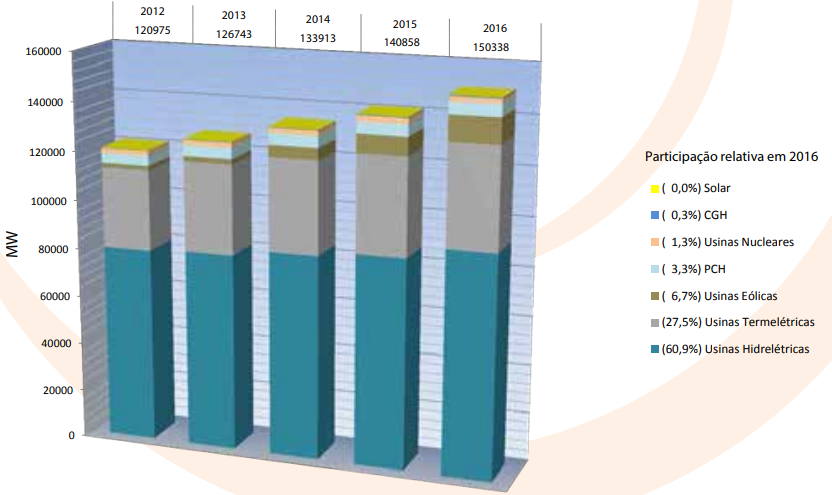
\includegraphics[width=0.9\textwidth, keepaspectratio=true]{forma_energia}
	\centering
	\caption[Capacidade de instalada de geração elétrica no Brasil (MW)]{Capacidade de instalada de geração elétrica no Brasil (MW)}
	\fonte{\cite[p. 57]{epe-anuario}.}
	\label{fig:rede_convencional}
\end{figure}
\FloatBarrier

A necessidade de contornar os desafios da crescente demanda energetica insentiva a busca por fontes alternativas e limpas de energia. O Brasil 
possui 42,30\% de fontes renováveis da sua matriz energetica e esse número deve aumentar até 2021 onde alcançará a marca de 85,00\% (as hidroelétricas
estão inclusas nesse meio), segundo o Ministério de Minas e Energia. No Plano Decemal de Expansão de Energia (PDE) 2020, o gorveno brasileiro
assume que a sustentabilidade é a chave mestra para a expenssão de atividades de geração de energia elétrica. A \autoref{fig:fonte_energia} mostra
que o Brasil vem investindo ao passar dos anos em fontes limpas de energias. Contudo também mostra que o Brasil ainda é muito dependente das 
hidrelétricas que apesar de ser uma fonte limpa e renovável traz malefícios como as grandes áreas alagadas em volta da represa, impactando no
ciclo de vida das espécies e obriga populaões ribeirinhas a migrarem, isso mostra que não basta apenas ter fontes limpas
e renováveis de energia, é necessário buscar melhorias como as Smart Grids e técnicas como de Smart metering.

\begin{figure}[h!]
	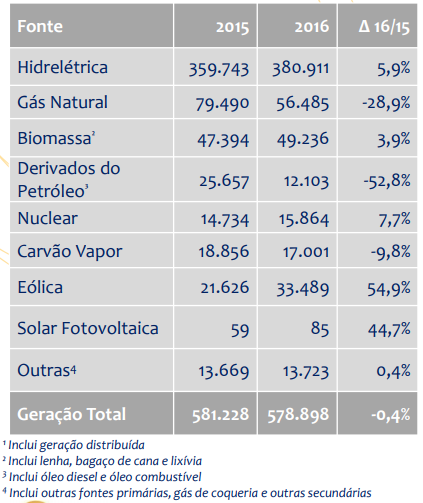
\includegraphics[width=0.7\textwidth, keepaspectratio=true]{fontes_energia}
	\centering
	\caption[Fontes de geração de energia elétrica (GWh)]{Fontes de geração de energia elétrica (GWh)}
	\fonte{\cite[p. 35]{epe-balanco}.}
	\label{fig:fonte_energia}
\end{figure}
\FloatBarrier

As chamadas redes inteligentes de transmissão e distribuição de energia, smart grid, tem como objetivo conectar unidades descentralizadas de geração
grande e pequena com o consumidor final. Assim nessa ideia o fluxo de energia se comunica de uma maneira bidirecional, a energia que é tradicionalmente
gerada e distribuidas pelas concessionárias poderá ser gerada e integrada as redes elétricas apartir de unidades consumidoras. O grande pilar dessa 
tecnologia são os sensores instalados ao longo da rede elétrica que constantemente estão enviando informações referente ao consumo a concessionária,
possibilitando um planejamento mais eficiente da rede. Aliado aos sensores na rede elétrica o consumidor recebe um medidor inteligente que também
é integrado com a concessionária em tempo real.

\begin{figure}[h!]
	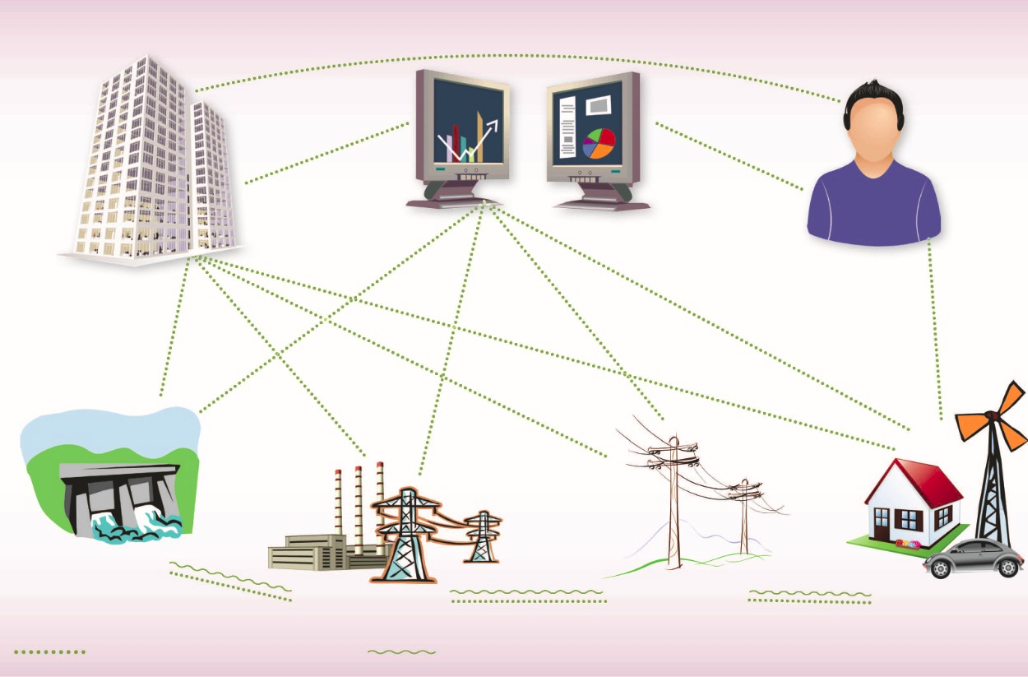
\includegraphics[width=0.7\textwidth, keepaspectratio=true]{rede_smartgrid}
	\centering
	\caption[Smart Grid,comunicação inteligente entre todos os usuários]{Smart Grid,comunicação inteligente entre todos os usuários}
	\fonte{\cite{smart-grid}.}
	\label{fig:rede_smartgrid}
\end{figure}
\FloatBarrier

O trabalho apresentará uma forma barata e eficiente de monitorar a energia elétrica de uma residência em tempo real, possibilitanto ao usuário
possuir informações valiosas a todo momento. O trabalho fará um paralelo com algumas das várias possibilidades de medição de consumo e monitoramento
de energia, provando que através da prática de gerenciamento e monitoramento de energia é possível conscientizar o usuário do mau uso da energia elétrica.
Então a partir desse dispositivo será possível entender como e onde a energia está sendo gasta, possibilitando mais informações ao usuário e ajudando para
que ele tome as precauções certas para economizar.

O trabalho será dividido da seguinte maneira: No \autoref{ch:cap2}


% Exemplo de citação direta com menos de três linhas. Como "o mercado de energia elétrica está baseado em tarifas fixas e limitações de informações em tempo real sobre gerenciamento da rede e da carga" \cite[p. 15]{cgee}, o consumidor acaba, então, não tendo como optar por fornecimentos elétricos mais adequados. 


\section{Uma subseção explicativa}

Lorem ipsum, uma citação direta 

\begin{citacao}[brazil]
[...] redes elétricas que podem, de forma inteligente, integrar o comportamento e as ações de todos os usuários conectados a ela, como geradores, consumidores e os que desempenham as duas funções, para entregar, eficientemente, um fornecimento de eletricidade sustentável, econômico e seguro \cite[p. 51, tradução livre]{yu2011new}.
\end{citacao}

Para compreender melhor as grandes mudanças e os benefícios gerados pelas \textit{Smart Grids} no contexto do fornecimento elétrico, a \autoref{tab-comparativa} traz um breve comparativo entre as redes tradicionais e as redes inteligentes.

\begin{table}[!ht]
\centering
\resizebox{\textwidth}{!}{%
\begin{tabular}{ll}
\hline
\multicolumn{1}{c}{\textbf{Redes Elétricas Tradicionais}} & \multicolumn{1}{c}{\textbf{Redes Elétricas Inteligentes}}                 \\ \hline
\rowcolor[HTML]{DDDDDD} 
Eletromecânica, estado sólido                             & Digital/Microprocessadores                                                \\
Unidirecional e localmente bidirecional                   & Global/comunicação bidirecional integrada                                 \\
\rowcolor[HTML]{DDDDDD} 
Geração centralizada                                      & Acomoda geração distribuída                                               \\
{Controle, monitoramento e proteção limitados}  & WAMPAC, proteção adaptativa \\
\rowcolor[HTML]{DDDDDD} 
"Cega"                                                    & Auto-monitoramento                                                        \\
Recuperação manual                                        & Auto-reconfigurável                                                       \\
\rowcolor[HTML]{DDDDDD} 
Checagem manual de equipamentos                           & Monitoração remota de equipamentos                                        \\
Sistema de controle de contingências limitado             & Sistema de controle pervasivo                                             \\
\rowcolor[HTML]{DDDDDD} 
Confiabilidade estimada                                   & Confiabilidade preditiva                                                 
\end{tabular}%
}
\caption{Comparação entre redes elétricas convencionais e redes elétricas inteligentes}
\label{tab-comparativa}
\fonte{\cite[p. 28, tradução nossa]{ali2013smart}}
\end{table}

\section{Trabalhos Relacionados}
\lipsum[1-1]

\section{Motivação}
O que lhe motiva a realizar este trabalho.

\section{Objetivos}
Objetivo geral e específicos.

\section{Estrutura do Trabalho}
Este trabalho apresenta uma introdução sobre o tema, mostrando os fatores que motivam a implantação da ideia, além da justificativa e dos objetivos. Em sequência, o \autoref{ch:cap2} aborda (...). O \autoref{ch:cap3}, por sua vez, explica a metodologia para ..., enquanto o \autoref{ch:cap4} trata de (...). O \autoref{ch:cap5} apresenta (...). Por fim, o \autoref{ch:cap6} traz as principais conclusões e contribuições deste trabalho.